% !TeX program = lualatex
%% La primera línea es un mapping entre la directiva TeX y el motor de compilación que utiliza VimTeX
%%% clase del documento
\documentclass{clase_tfm}[2023/04/21]
\begin{document}

%%% titulo y dedicatoria
\frontmatter
\pagenumbering{Roman} % números romanos en mayúsculas (polyglossia no tiene todavía opción para hacerlo automáticamente en español) 

\titlehead{{\Large \unienc} \\ 
\etsiienc \\
\dirinst \\
\cpinst}

\subject{\titproy}
\title{\titenc}
\author{Autor: \nomautor}
\date{\today}
\publishers{Tutor: \nomtutor}

\dedication{A mis padres \\
A mis amigos \\
A mi tutor.}

\maketitle


%%% resumen y agradecimientos
\addchap{Agradecimientos}
\addchap{Resumen}
\lettrine{D}{esde la aparición de los primeros láseres} a principios de $1960$, estos complejos sistemas ópticos han encontrado multitud de aplicaciones tanto en investigación científica como en la industria tecnológica, transforman diversos campos gracias a sus increíbles propiedades físicas y gran versatilidad. En el ámbito científico, los láseres se utilizan constantemente en espectroscopia, permitiendo analizar la composición de materiales a escala molecular o la estructura de microorganismos como bacterias y virus. 

Sus aportaciones en física y química, que han llegado a reunir más de una decena de Premios Nobel, han conseguido alcanzar hitos extraordinarios, relacionados con disciplinas como la óptica cuántica, la óptica ultrarrápida o la nanotecnología. En la industria, se han convertido en instrumentos indispensables de corte, soldadura y marcado de materiales con alta precisión. En las telecomunicaciones, son cruciales en la transmisión de información a través de fibras ópticas, mejorando la velocidad y la eficacia de las comunicaciones. En medicina, muchos procedimientos quirúrgicos emplean sistemas láser para realizar operaciones, además de estar presentes también en el diagnóstico clínico y tratamiento de enfermedades como diferentes tipos de cáncer.

En este Trabajo Fin de Máster, se estudia la interacción de un armónico de alto orden (\acrshort{hoh}) con un plasma amplificador de radiación ultravioleta extrema o rayos X blandos (\acrshort{xuv}) formado por iones de kriptón altamente ionizados (\ce{Kr^{8+}}), responsables de la amplificación. Mediante la realización de simulaciones numéricas, el objetivo es reproducir las condiciones y resultados obtenidos experimentalmente, ayudando en la comprensión de los distintos fenómenos físicos que participan en el proceso de amplificación del armónico.

Estas simulaciones están centradas en la utilización del código Dagon\autocite{Oliva2017}, encargado de modelizar la amplificación tridimensional del armónico inyectado a través de una columna de plasma, introduciendo las ecuaciones de Maxwell-Bloch para su resolución numérica. El código fue desarrollado en el Instituto de Fusión Nuclear \enquote{Guillermo-Velarde} (IFN-GV) de la Escuela Técnica Superior de Ingenieros Industriales (ETSII), en la Universidad Politécnica de Madrid (UPM), a partir del esfuerzo realizado por el Dr. Eduardo Oliva Gonzalo ---tutor y guía del trabajo--- para estudiar láseres de rayos X blandos basados en plasmas (\acrshort{sxrl}).

Los antecedentes que motivaron la aparición de este trabajo fueron varios experimentos\autocite{Tuitje2020,Depresseux2015} llevados a cabo en el \emph{\acrfull{loa}}, situado en París, donde un gas de kriptón a alta presión es fuertemente ionizado mediante un sistema de varios pulsos láser infrarrojos, formándose un canal de plasma capaz de amplificar un haz de rayos X blandos ($\lambda=\qty{32.8}{nm}$). Estos experimentos buscaban reducir la duración del pulso de radiación ultravioleta producido, además de medir propiedades como la evolución temporal de los fotones o las distribuciones de iones y electrones en el interior del canal de plasma. 

Sin embargo, algunos aspectos relacionados con las curvas de intensidad y fase del haz amplificado no se entendían correctamente al principio. El esquema presentado en este proyecto consiste en modificar la distribución de \ce{Kr^{8+}} en la columna de plasma, introduciendo en Dagon parámetros que permitan controlar la región de abundancia del ión en el interior del medio activo. De esta manera, es posible estudiar sistemáticamente los efectos que tienen cuestiones como la anchura del canal con presencia de \ce{Kr^{8+}} sobre la amplificación, intentando ajustarse a las observaciones experimentales.

A partir de las imágenes obtenidas en las simulaciones ejecutadas, ha sido posible mejorar el entendimiento de la amplificación resultante en las distribuciones de intensidad y fase mencionadas, estudiando la influencia de la geometría de la frontera que alberga el ión \ce{Kr^{8+}} en su interior, variando parámetros como su amplitud en dirección radial a lo largo de la longitud de la columna de plasma.

Especialmente, el postprocesamiento de las imágenes ha revelado la capacidad de replicar perfectamente el efecto de la sobreionización inicial producida durante la formación del canal de plasma, responsable de la formación de un valle en el perfil radial de intensidad del haz a la salida del canal. Además, la tendencia de esta curva también ha podido adaptarse razonablemente a los resultados del laboratorio, así como la profundidad entre máximos y mínimos del perfil radial de fase de los fotones.

A pesar de esto, el acuerdo conseguido entre simulación y experimento todavía necesita mejorar la precisión, haciendo énfasis en la densidad electrónica o en otros aspectos de la concentración de \ce{Kr^{8+}} dentro del canal de plasma, que pudieran reducir las discrepancias observadas. Nuevas investigaciones y proyectos deberán concentrar sus esfuerzos en proponer nuevas modificaciones en la distribución de iones y electrones, partiendo de las observaciones realizadas en trabajos anteriores.

De este modo, en el futuro podrían utilizarse estas fuentes de radiación para la diagnosis y reconstrucción de imágenes en tres dimensiones, sustituyendo tal vez grandes instalaciones ---empleadas, por ejemplo, en los láseres de electrones libres (\acrshort{fel})--- cuya operación resulta más costosa y compleja de mantener. 

En definitiva, este trabajo está integrado dentro de una amplia línea de investigación dedicada a comprender la amplificación de haces de rayos X blandos mediante plasmas densos que interaccionan con pulsos de armónicos de alto orden. Los resultados obtenidos demuestran la posibilidad de reproducir mediante simulaciones numéricas aspectos fundamentales de la intensidad y fase del pulso ultravioleta extremo a la salida del medio activo. 

\begin{table}[htpb]
    \begin{tabular}{l}
        \textbf{Palabras Clave} \\
        \midrule
         Canal de plasma, láser XUV, armónicos de alto orden, código Dagon, Maxwell-Bloch. 
    \end{tabular}
\end{table}

\begin{table}[htpb]
    \begin{tabular}{ll}
        \textbf{Códigos UNESCO} & \\
        \midrule
         220910 & Láseres \\
         220909 & Radiación infrarroja \\
         220212 & Rayos X \\
         220702 & Iones atómicos \\
         220410 & Física de plasmas \\
         220407 & Ionización 
    \end{tabular}
\end{table}


%%% indice general
\tableofcontents

%%% cuerpo del documento
\mainmatter

\chapter{Introducción}\label{cap:1}
\lettrine{E}{n este capítulo, la misión principal} consiste en presentar, de forma clara y concisa, los fundamentos básicos que están detrás del presente Trabajo Fin de Máster. El contexto histórico aparece constantemente durante este proyecto, así como los protagonistas principales, sus descubrimientos y sus aportaciones más importantes en el marco del estudio realizado. De esta manera, se pretende que los futuros lectores puedan comprender las motivaciones y objetivos básicos perseguidos durante la ejecución del mismo.

En primer lugar, este trabajo está integrado dentro de una línea de investigación supervisada por el Dr. Eduardo Oliva Gonzalo ---ubicado en el Instituto de Fusión Nuclear \enquote{Guillermo Velarde} (IFN-GV)---, dedicada principalmente al análisis y modelización de la interacción láser-plasma para la generación y amplificación de rayos X blandos o radiación ultravioleta extrema. Los inicios de la investigación se remontan al comienzo de la tesis doctoral del Dr. Eduardo Oliva\autocite{Oliva2010a}, para unos años después, en el año $2015$, comenzar a dirigir los primeros Trabajos Fin de Grado y Fin de Máster. Los trabajos realizados por Alba Guiomar Verdejo, Marina Ruiz Izu o Santiago López García guardan una relación estrecha con este trabajo, siendo la temática de este trabajo en cierta forma una continuación de estos, o aquellos antecesores de este.

Además, este estudio ha sido realizado en paralelo a las prácticas curriculares, supervisadas nuevamente por el Dr. Eduardo Oliva y revisadas por el Dr. Manuel Cotelo Ferreiro ---también ubicado en el IFN-GV---, destinadas principalmente a realizar tareas de modelización de armónicos de alto orden en plasmas mediante la escritura o modificación de programas, para después obtener y procesar las imágenes resultantes de las simulaciones. Los resultados y conclusiones presentados en los capítulos \S\ref{cap:4} y \S\ref{cap:5}, así como gran parte del trabajo de documentación y estudio realizado para la redacción, son fruto del tiempo empleado durante este periodo de prácticas.

En segundo lugar, los futuros lectores de este trabajo sentirán la necesidad de preguntarse por el título del mismo, su significado conjunto y el de los conceptos individuales que constituyen el estudio. La finalidad de este primer capítulo introductorio es satisfacer parcialmente estas preguntas a cerca de la naturaleza del TFM para después, en los capítulos \S\ref{cap:2} y \S\ref{cap:3}, terminar de presentar las ideas básicas que subyacen el proyecto y comenzar el análisis de los resultados en el capítulo \S\ref{cap:4}. Sin embargo, para orientar anticipadamente a los lectores, se presentan a continuación ---sin entrar en detalle--- las líneas básicas que aparecerán más detalladas posteriormente.

\begin{itemize}
  \item Láseres. A las escalas de energía e intensidad empleadas en la mayor parte de aplicaciones del mundo, es suficiente emplear un tratamiento clásico de la radiación láser. Dentro de este marco, es un sistema que produce ondas electromagnéticas con unas propiedades ópticas especiales, siendo el protagonista de una infinidad de aplicaciones científicas y tecnológicas como, por ejemplo, la fusión por confinamiento inercial o los interferómetros modernos. La sección \S\ref{sec:1.1} desarrolla estos sistemas en mayor profundidad.
  \item Rayos X blandos. También llamados radiación ultravioleta extrema, del inglés \emph{\acrfull{xuv}}, tienen longitudes de onda comprendidas entre los \qty{2}{nm} y \qty{20}{nm}. Los fenómenos ondulatorios que aparecen cuando una onda electromagnética interacciona con la materia ocurren gracias a que comparten longitudes de onda y tamaños característicos similares, motivando la utilización de radiación \acrshort{xuv} para observar escalas nanométricas, comunes por ejemplo entre familias de virus.
  \item Pulsos ultracortos y ultraintensos. Para visualizar correctamente escalas con un determinado tamaño, es necesario que la onda electromagnética deposite sobre la materia la cantidad de energía necesaria durante un intervalo de tiempo que permita obtener una resolución adecuada antes de inutilizar o destruir la muestra. La aparición a mediados de la década de los años ochenta de la técnica \acrshort{cpa}, acrónimo que significa \emph{\acrlong{cpa}}, desarrollada por Donna Strickland y Gérard Mourou\autocite{Strickland1985}, comenzó una nueva era de láseres capaces de proporcionar pulsos con energías de $\sim\unit{mJ}$ y $\sim\unit{fs}$ de duración, claves en un gran número de aplicaciones mencionadas a lo largo de este trabajo, incluido este mismo proyecto.
  \item Plasmas. El interés que despiertan está relacionado con la capacidad de ciertas especies de iones en plasmas densos de actuar como un medio amplificador de radiación \acrshort{xuv} en láseres basados en plasmas, especialmente cuando esta radiación son armónicos de alto orden. Las propiedades físicas y el comportamiento óptico de este estado de la materia aparece durante la sección \S\ref{sec:1.2}. 
  \item Armónicos de alto orden. Aparecen nombrados en la terminología inglesa mediante el acrónimo \emph{\acrfull{hoh}}. La generación de armónicos de alto orden, también acrónimo de \emph{\acrfull{hhg}}, permite obtener armónicos ---ondas puras---, de radiación coherente con duraciones extremadamente cortas (pueden llegar a obtenerse pulsos de attosegundos) mediante la interacción de un láser muy intenso con un blanco generalmente gaseoso o sólido. Aunque individualmente son fuentes de radiación \acrshort{xuv} coherente con propiedades ópticas de gran importancia, explicadas en la sección \S\ref{sec:1.3}, combinar la inyección de armónicos de alto orden en plasmas densos permite obtener pulsos láser con características similares a los láseres de electrones libres (\acrshort{fel}), de mejores prestaciones que las demás fuentes por separado, pero reduciendo el tamaño y coste de las instalaciones. 
\end{itemize}

La síntesis de estos conceptos dan como resultado la posibilidad de utilizar armónicos de alto orden como una fuente de radiación \acrshort{xuv} coherente amplificada mediante su interacción con un plasma muy denso. Los capítulos \S\ref{cap:2} y \S\ref{cap:3} presentan esta conjunción de elementos en mayor profundidad, estando el plasma objeto de análisis durante este trabajo formado a partir de un gas de kriptón fuertemente ionizado, a través del cual viaja un armónico de alto orden para su amplificación y mejora de sus propiedades ópticas. 

Las discrepancias existentes entre, por una parte, los múltiples experimentos llevados a cabo anteriormente y, por otro lado, las simulaciones numéricas, respecto a las características de la emisión \acrshort{xuv} obtenida, son el centro de estudio del capítulo \S\ref{cap:4} y, esencialmente, el objetivo principal perseguido es explicar y reducir estas diferencias introduciendo modificaciones en los códigos disponibles para analizar, posteriormente, los resultados observados.

\section{Láser}\label{sec:1.1}
En la actualidad, los láseres están presentes en una infinidad de aplicaciones científicas y tecnológicas. Muchas aplicaciones son bien conocidas por la mayoría de la población general: procedimientos quirúrgicos en medicina y cirugía, mediciones de muy alta precisión, reconstrucción de imágenes tridimensionales ---conocida como holografía---, giroscopios de alta sensibilidad, escáneres de supermercados, reproductores CD, DVD y Blue-Ray, soldaduras y perforaciones de materiales, trazado de líneas rectas en superficies y topografía, litografía de materiales, telecomunicaciones y fibra óptica, y así sucesivamente.

En los primeros años de desarrollo, en la década de $1960$, existía un gran escepticismo \autocite{SanchezRon2022} sobre su aparición, siendo muchas las personas que calificaban estas tecnologías emergentes como \enquote{una solución en busca de un problema}. Desde entonces han ido apareciendo muchos de estos supuestos \enquote{inconvenientes}, como los ejemplos expuestos, hasta convertir el láser en una parte fundamental de la ciencia y la tecnología de nuestro tiempo.  

Las palabras láser y máser son acrónimos, respectivamente, de \emph{\acrfull{laser}} (amplificación de luz por emisión estimulada de radiación) y de \emph{\acrfull{maser}} (amplificación de microondas por emisión estimulada de radiación). Los orígenes teóricos de ambas técnicas, cuyos fundamentos aparecerán explicados durante la sección \S\ref{sec:1.1.1}, tienen como cimientos el contenido de dos artículos de Einstein\autocite{Einstein1916,Einstein1916a}, publicados en $1916$, acerca del descubrimiento de la emisión espontánea.

Sin embargo, la aparición de los primeros instrumentos no sucedió hasta la década de $1950$. Los principales responsables de semejante logro fueron, de forma independiente, Aleksandr M. Prokhorov y Nikolai G. Basov, del Instituto Lebedev de Física de Moscú, y Charles Townes, de la Universidad de Columbia, Nueva York, que recibieron el Premio Nobel de Física en $1964$. Especialmente meritorio fue el análisis de Joseph Weber \autocite{Weber1953a} durante el año $1953$, en el que reflexionó sobre la posibilidad de obtener una emisión estimulada a partir de una inversión de población electrónica, concepto que también aparecerá en la sección \S\ref{sec:1.1.1}.

En $1952$, durante una conferencia \autocite{SanchezRon2014} sobre radio-espectroscopía en la antigua Academia de Ciencias de la URSS, Basov y Prokhorov describieron el principio del máser, aunque la primera publicación tardó dos años en llegar \autocite{Basov1954}. Además, Basov construyó un máser como parte de su tesis doctoral, unos meses después de que Townes hiciese la primera demostración experimental del máser, que había participado activamente durante la Segunda Guerra Mundial en el desarrollo del radar, mientras trabajaba en los Laboratorios Bell.

Para lograr semejante tarea, Townes necesitó la colaboración de Herbert J. Zeiger, un joven doctor en física que había trabajado en técnicas de haces moleculares, y un doctorando, James P. Gordon. El primer máser apareció el $5$ de mayo de $1954$ empleando un gas de moléculas de amoniaco\autocite{Gordon1954}, consiguiendo una emisión coherente de microondas; esto es, radiación altamente concentrada, de una longitud de onda. 

Las ideas de extender la emisión a longitudes de onda en la luz visible no tardaron en proliferar entre los físicos, incluido el propio Townes (también Basov y Prokhorov), colaborando con su cuñado, Arthur Schawlow, un físico de los Laboratorios Bell. En un artículo de $1958$\autocite{Schawlow1958}, mostraron cómo se podría un láser, idea que patentaron dos años más tarde. La carrera por la construcción del láser se aceleró a partir de entonces, ganándola Theodore Maiman, de los Hughes Research Laboratories de Malibu (California), que consiguió poner en funcionamiento un láser de rubí (de estado sólido) \autocite{Maiman1960} el $16$ de mayo de $1960$.

Queda claro que los logros alcanzados por los láseres, y las expectativas puestas en ellos, no conocían, ni conocen, límites. De hecho, como se adelantaba al comenzar esta sección \S\ref{sec:1.1}, todos los desarrollos producidos durante las primeras décadas fueron superados posteriormente. Por ejemplo, su aplicación en espectroscopía han permitido conocer mucho mejor las propiedades de muchas moléculas con estructuras más complejas que los propios átomos. Nuevas especialidades como la óptica cuántica aparecieron a partir del láser, y trabajos como los de Claude Cohen-Tannoudji \autocite{Dalibard1985}, Steve Chu \autocite{Chu1989,Chu1986}, William Phillips \autocite{Migdall1985} y Arthur Ashkin \autocite{Ashkin1978,Ashkin1970} para atrapar y enfriar átomos con láseres, demuestran ampliamente esta capacidad de superación.

\subsection{Interacción radiación-materia}\label{sec:1.1.1}

\begin{equation}\label{eq:1.1}
  \nu_{0} = \frac{E_{2}-E_{1}}{h}
\end{equation}

\subsection{Propiedades ópticas}\label{sec:1.1.2}
La radiación emitida por un láser está caracterizada principalmente por una alta monocromaticidad, coherencia, direccionalidad e intensidad. A estas propiedades puede añadirse una quinta relacionada con la duración de la emisión\autocite{Svelto2010}. Esta última hace referencia a la capacidad de generar pulsos de muy corta duración, propiedad que, aunque menos fundamental, tiene gran importancia en muchas aplicaciones. 

\paragraph{Monocromaticidad}\label{par:1.1.2.1}
De forma simplificada, esta propiedad se debe fundamentalmente a dos motivos: en primer lugar, solamente una onda electromagnética de frecuencia $\nu_0$ dada por \eqref{eq:1.1} puede ser amplificada y, en segundo lugar, como los esquemas de espejos utilizados forman una cavidad resonante, las oscilaciones pueden producirse únicamente a las frecuencias de resonancia de esta cavidad. Esta última circunstancia implica que el ancho de banda $\Delta\nu$ de la emisión láser es habitualmente mucho menor ---hasta diez órdenes de magnitud--- que el ancho de banda observado en la transición $2\rightarrow 1$ durante la emisión espontánea asociada.

Por ejemplo, las últimas propuestas de láseres de Fabry-Perot para la fabricación de circuitos integrados \autocite{Tran2022}, emplean frecuencias de \qty{300}{THz} ($\lambda = \qty{980}{nm}$) con anchos de banda $\Delta\nu = \qty{10}{kHz}$, resultando una anchura relativa para la frecuencia de emisión $\Delta\nu/\nu = 3,33\times 10^{-11}$. El espectro de la emisión láser tiene una alta pureza, como ilustra la Figura \ref{fig:ch1_amplif}, consiguiéndose reducir la dispersión a través de un medio de propagación dado y mejorando la focalización del haz, ya que el índice de refracción depende de la longitud de onda emitida.

\begin{figure}[ht!]
  \centering
  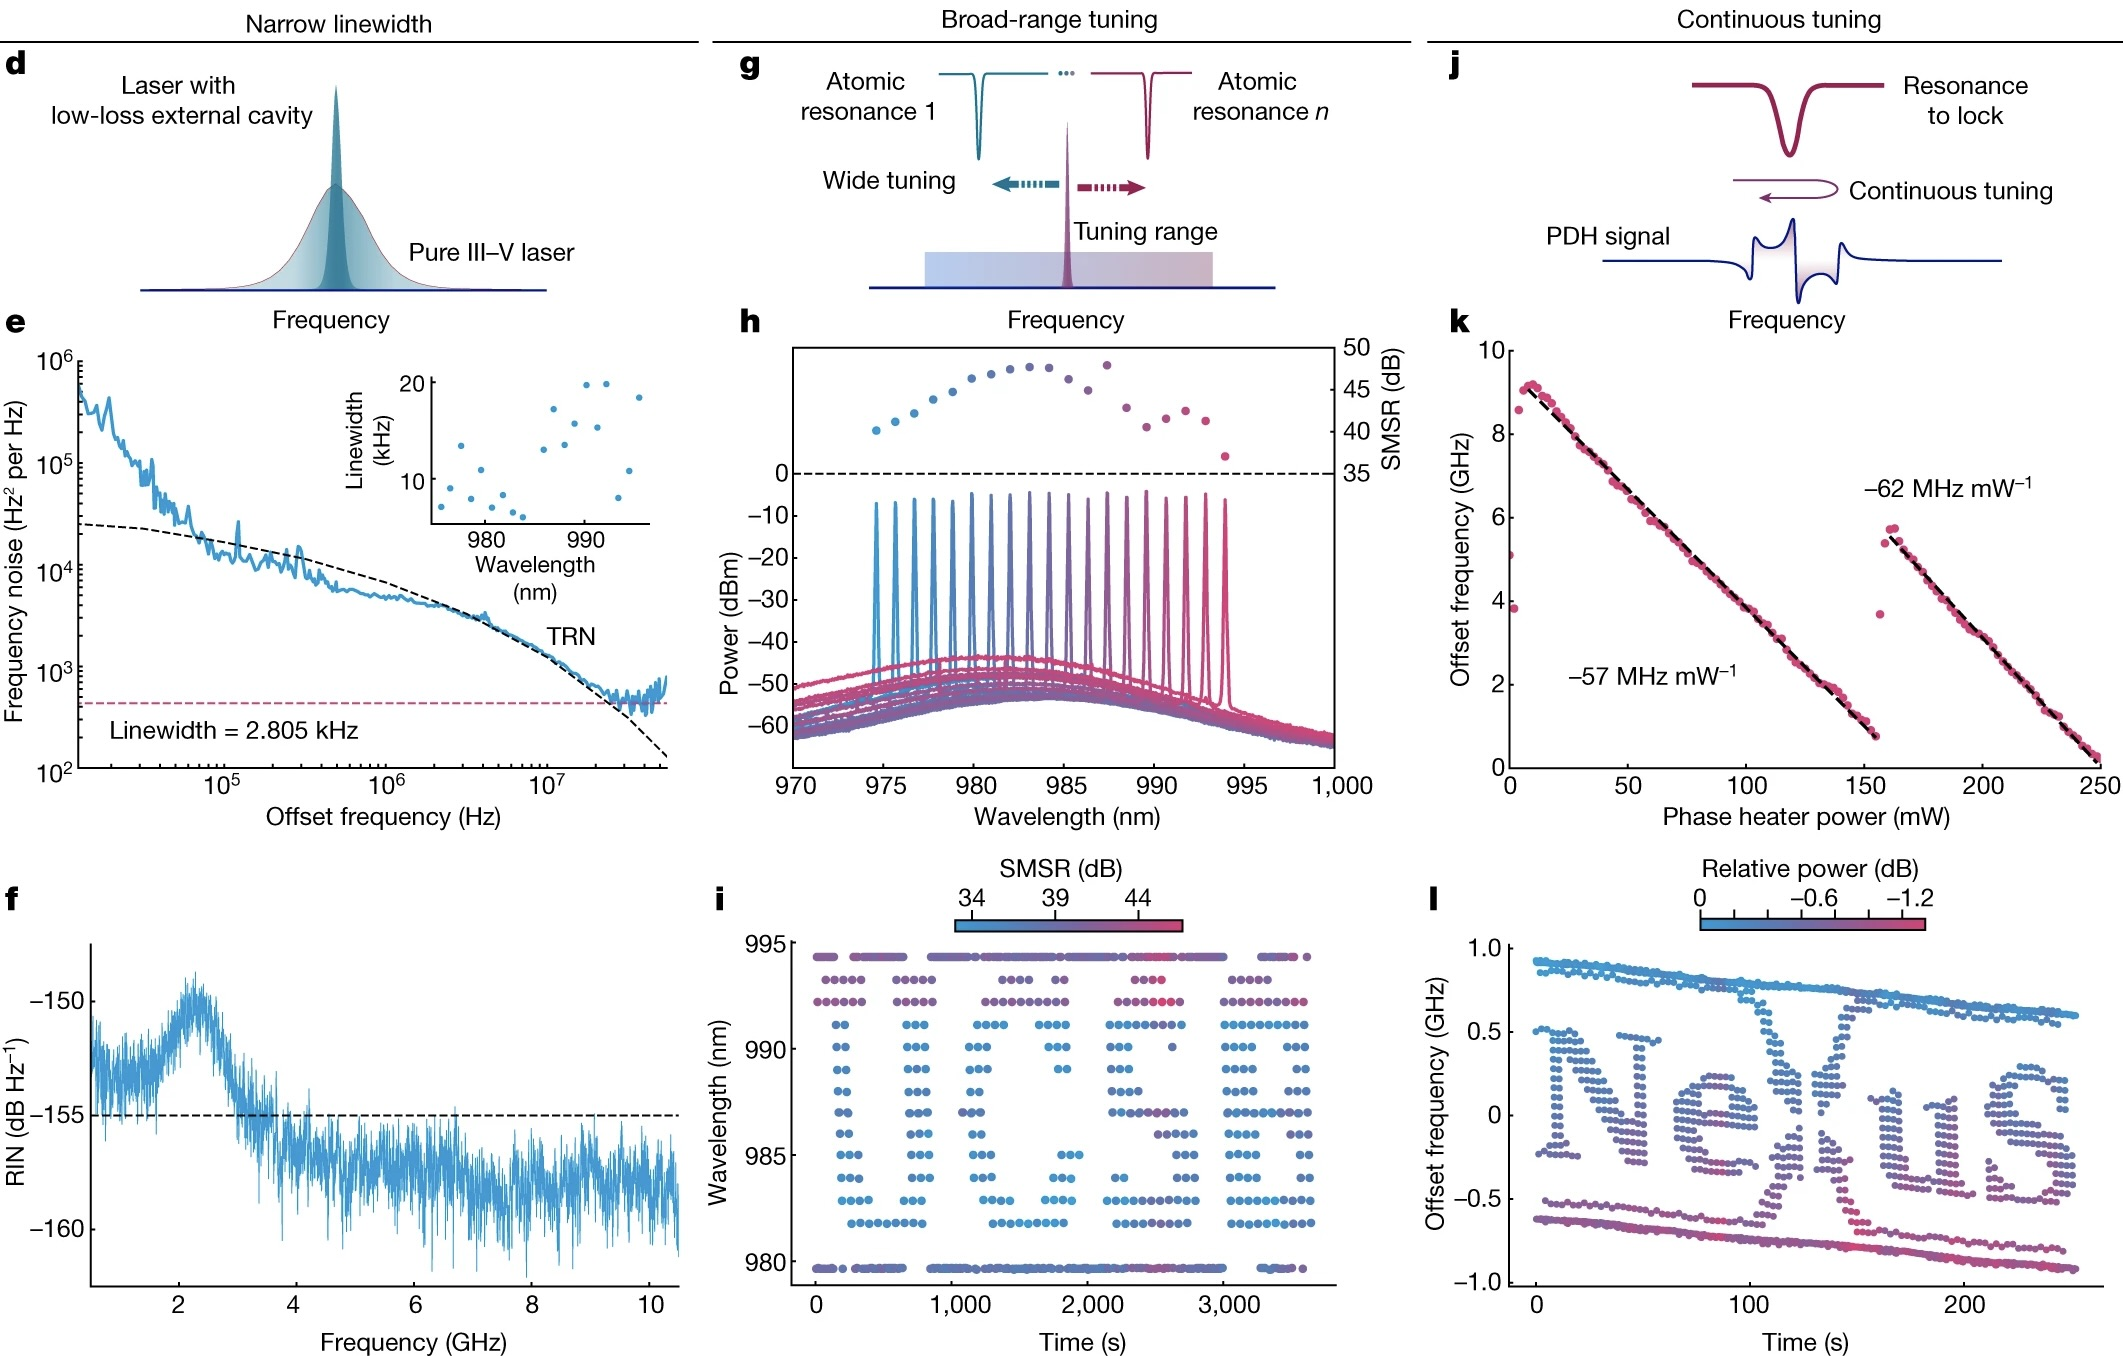
\includegraphics[width=\textwidth]{Figuras/ch1_amplif.png}
  \caption{Espectro de emisión del láser empleado en la propuesta\autocite{Tran2022}. \textbf{b}, Esquema del láser y sus elementos. \textbf{d}, Ancho de banda conseguido con la cavidad resonante. \textbf{e}, Ruido en la frecuencia del espectro de emisión. \textbf{g}, Frecuencias de resonancia. \textbf{h}, Longitudes de onda de operación.}
  \label{fig:ch1_amplif}
\end{figure}

En realidad, la longitud de onda de la transición láser admite ---por el principio de incertidumbre de Heisenberg--- frecuencias de excitación distintas a la ecuación \eqref{eq:1.1}, tal que $\nu_0\rightarrow\nu_0 + \delta\nu$. La magnitud de $\delta\nu$ es proporcional a la constante de Planck $h = \qty{6,626e-34}{J.s}$, siendo entonces extremadamente pequeña la variación introducida en el ancho de banda de la emisión láser debido a este fenómeno. 

Además, Schawlow y Townes demostraron que la anchura de banda mínima de un láser es la anchura de banda de la cavidad resonante dividida por dos veces el número de fotones $\langle n\rangle$ en el interior de la cavidad, límite conocido como \emph{\acrfull{sql}}. Sin embargo, existen grupos de investigación\autocite{Liu2021} que sugieren la posibilidad de utilizar circuitos superconductores para superar el \acrshort{sql} por un factor $\sim \xval{n}$ e incluso $\sim \xval{n}^{2}$, aproximándose al denominado \emph{límite de Heisenberg}.

\paragraph{Coherencia}\label{par:1.1.2.2}
A primer orden, el concepto de coherencia de una onda electromagnética introduce dos conceptos, llamados coherencia espacial y temporal\autocite{Svelto2010}.

Para definir la coherencia espacial, basta con imaginar dos puntos $P_1$ y $P_2$ situados en el mismo frente de onda, en un instante inicial, de una onda electromagnética determinada, siendo $E_1(t)$ y $E_2(t)$ las amplitudes del campo eléctrico en dichos puntos. Por definición, el desfase entre ambos campos en ese instante es cero. Ahora bien, si en cualquier instante posterior, el desfase entre ambos mantiene un valor nulo, entonces se dice que ambos puntos tienen una coherencia perfecta. Si esto ocurre para cualquier par de puntos del frente de onda, entonces se dice que la onda tiene \emph{coherencia espacial perfecta}. En la práctica, para un punto $P_1$, el punto $P_2$ tiene que estar en un área muy próxima a $P_1$ para mantener una buena correlación entre ambas fases. En estos casos, existe una \emph{coherencia espacial parcial} y, para cualquier punto $P$, puede definirse un área de coherencia $S_{c}(P)$ apropiada.

Para definir la coherencia temporal, se supone el campo eléctrico de la onda anterior en un punto $P$, pero en dos instantes de tiempo $t$ y $t+\tau$. Si para un determinado intervalo $\tau$, el desfase entre las dos ondas se mantiene constante para cualquier instante de tiempo $t$, entonces se dice que tienen coherencia temporal durante el intervalo $\tau$. Si esto ocurre para cualquier $\tau$, la onda electromagnética tendrá una \emph{coherencia temporal perfecta}. En la práctica, el desfase puede mantenerse durante cualquier intervalo de tiempo $\tau$, tal que $0<\tau<\tau_0$, en cuyo caso la onda tiene \emph{coherencia temporal parcial} con un tiempo de coherencia $\tau_0$. En experimentos recientes\autocite{Zhou2020}, el láser de electrones libres (\acrshort{fel}) del \emph{\acrfull{lcls}} ha proporcionado pulsos de rayos X duros (\qty{60}{µJ}, \qty{3}{fs}) con un tiempo de coherencia parcial de $\tau_0 = \qty{174,7}{as}$ (\qty{1}{as} = \qty{e-18}{s}). La Figura \ref{fig:ch1_coher} muestra los tiempos de coherencia obtenidos en dicho experimento. 

Es importante mencionar que ambos conceptos de coherencia son independientes. De hecho, pueden darse casos de ondas con buena coherencia espacial y mala coherencia temporal, o viceversa. Además, como se ha comentado inicialmente, estas propiedades aparecen cuando se estudia el grado de coherencia de la onda a primer orden. Esta caracterización, en general, consiste en medir por ejemplo, mediante un interferómetro de Young, un elevado número de veces el campo eléctrico en dos puntos distintos del espacio $\symbf{r}_1$ y $\symbf{r}_2$ para dos instantes de tiempo $t_1$ y $t_2$ de un intervalo $T$, definiéndose el \emph{grado de coherencia de primer orden} como
\begin{equation}\label{eq:1.2}
  \gamma^{(1)}(\symbf{r}_{1},\symbf{r}_{2},t_{1},t_{2}) = \frac{\langle E(\symbf{r}_{1},t_{1})E^{*}(\symbf{r}_{2},t_{2}\rangle)}{\langle E(\symbf{r}_{1},t_{1})E^{*}(\symbf{r}_{1},t_{1}) \rangle^{1/2} \langle E(\symbf{r}_{2},t_{2})E^{*}(\symbf{r}_{2},t_{2}) \rangle^{1/2}},
\end{equation}
con $E^{*}$ el complejo conjugado del campo eléctrico. En esencia, la ecuación \eqref{eq:1.2} \enquote{ensambla} el valor medio de las mediciones realizadas para el campo eléctrico y las normaliza, permitiendo medir simultáneamente coherencia espacial y temporal de la onda.

\begin{figure}[ht!]
  \centering
  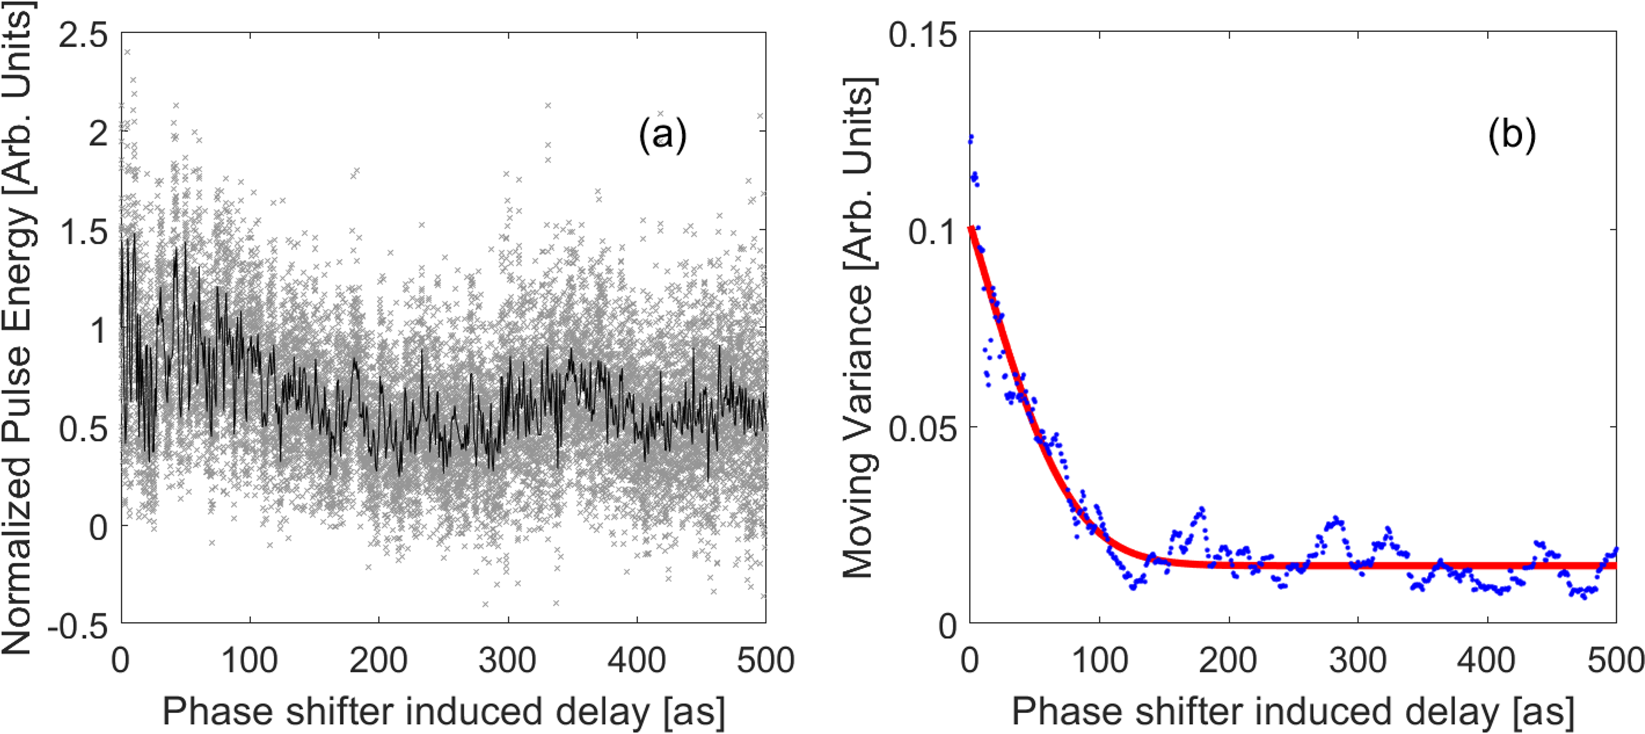
\includegraphics[width=0.8\textwidth]{Figuras/ch1_coher.png}
  \caption{Resultados experimentales del tiempo de coherencia medidos en el \acrshort{lcls}\autocite{Zhou2020}. \textbf{a}, Energía de los pulsos frente al retraso temporal. \textbf{b}, Cambios en la varianza respecto al retraso temporal.}
  \label{fig:ch1_coher}
\end{figure}

El concepto de coherencia de primer orden hace referencia a que la medición realizada contempla la correlación entre amplitudes de ondas --el campo eléctrico---, mientras que la coherencia de orden $n$ expresa la correlación entre los productos de orden $n$ del campo eléctrico. Por ejemplo, a segundo orden ---el cuadrado del campo eléctrico---, la medición encierra la información sobre la intensidad del campo, de manera que la \emph{función correlación de orden} $n$ sería $\Gamma^{(n)}(\symbf{r}_1,t_1,\ldots,\symbf{r}_n,t_n) = \langle E(\symbf{r}_1,t_1)E^{*}(\symbf{r}_1,t_1)\ldots E(\symbf{r}_n,t_n)E^{*}(\symbf{r}_n,t_n)\rangle$.

\paragraph{Direccionalidad}\label{par:1.1.2.3}
La emisión de un láser puede llegar a consistir en frentes de onda planos prácticamente ideales. La difracción es el único fenómeno ondulatorio que impone un umbral inferior en la divergencia del haz láser. El orden de magnitud del ángulo sólido $\Delta\Omega$ y el ángulo de divergencia $\Delta\theta$ dependen fundamentalmente de la longitud de onda $\lambda$ y el área de apertura $A$ de la emisión\autocite{Milonni1988} a través de la relación
\begin{equation}\label{eq:1.3}
    \Delta\Omega \approx \frac{\lambda^{2}}{A} \approx (\Delta\theta)^{2}.
\end{equation}
Para longitudes de onda en el rango óptico, por ejemplo, $\lambda = \qty{500}{nm}$, y con una superficie de salida de la cavidad habitual de $A = \qty{5}{mm^2}$, la relación \eqref{eq:1.3} proporciona una divergencia de $\Delta\theta = \sqrt{\qty{250000e-18}{m^2}/(\qty{25e-6}{m^2})} = \qty{0,1}{mrad}$. Con ángulos de divergencia similares a este ejemplo, que son habituales en láseres, como muestra la Tabla \ref{tab:1.1}, el llamado \emph{rango de Rayleigh} permite caracterizar la distancia recorrida $z$. En este rango, el ancho $w_0$ del haz láser se incrementa en un factor $\sqrt{2}$ en el plano transversal, siendo aproximadamente en este caso
\begin{equation}\label{eq:1.4}
    z\approx\frac{A}{\lambda} = \frac{\qty{5e-6}{m^2}}{\qty{500e-9}{m}} = \qty{10}{m}.
\end{equation}

Para áreas de apertura mayores, por ejemplo $A = \qty{5}{cm^2}$, la distancia aumenta hasta alcanzar $z = \qty{1}{km}$. Empleando menores longitudes de onda el rango sería incluso mayor, dando una idea de las largas distancias capaces de recorrer muchos láseres sin pérdida de direccionalidad.

\begin{table}[ht!]
  \centering
  \caption{Ángulos de divergencia típicos en láseres\autocite{Milonni1988}.}
  \begin{tabular}{ccc}
    \toprule
     Láser           & $\Delta\theta$ (\unit{mrad}) & $\Delta\Omega$ (\unit{sr}) \\
    \midrule
    \ce{He-Ne}      & $0,2-1$                                & $(0,1-3)\times 10^{-6}$ \\
    \midrule
    \ce{CO2}        & $1-10$                                  & $(3-300)\times 10^{-6}$ \\
    \midrule
    Rubí            & $1-10$                                  & $(3-300)\times 10^{-6}$ \\
    \midrule
    \ce{Nd{:}YAG}     & $1-20$                                & $(3-1300)\times 10^{-6}$ \\
    \midrule
    \ce{Nd{:}cristal} & $0,5-10$                              & $(1-300)\times 10^{-6}$ \\
    \bottomrule
  \end{tabular}
  \label{tab:1.1}
\end{table}

\paragraph{Luminosidad}\label{par:1.1.2.4}
Un haz de luz procedente de una fuente puede caracterizarse por la divergencia del haz $\Delta\Omega$, el tamaño de la fuente ---normalmente una superficie de área $A$---, el ancho de banda $\Delta\nu$ y la densidad de potencia de la emisión $P(\nu)$, es decir, la potencia por unidad de frecuencia del ancho de banda\autocite{Milonni1988}. A partir de estos parámetros, es interesante definir la \emph{luminosidad espectral} $\beta_{\nu}$ de la fuente como 
\begin{equation}\label{eq:1.5}
    \beta_{\nu} = \frac{P(\nu)}{A\Delta\Omega\Delta\nu} = \frac{I(\nu)}{\Delta\Omega},
\end{equation}
con $I(\nu)$ la intensidad espectral del haz de luz, de manera que también puede definirse $\beta_{\nu}$ como la intensidad espectral por unidad de ángulo sólido.

Para una fuente de radiación ordinaria, esta luminosidad puede estimarse directamente suponiendo la expresión de la densidad espectral de energía $\rho(\nu)$ de un cuerpo negro. Empleando la ecuación \eqref{eq:1.5} y la hipótesis del cuerpo negro ($\Delta\Omega=4 \pi$), resulta
\begin{equation}\label{eq:1.6}
    \beta_{\nu} = \frac{c \rho(\nu)}{4 \pi} = \frac{2 \nu^{2}}{c^{2}}\frac{h \nu}{\eu^{h \nu/kT}-1}.
\end{equation}
La temperatura de la superficie del sol es aproximadamente $T = \qty{5800}{K} \approx 20 \times \qty{300}{K}$. La mayoría de la emisión del sol está en la franja amarilla de la banda visible, de forma que $h\nu \approx \qty{2,5}{eV}$ ($\nu \approx \qty{5e14}{Hz}$ para un fotón en el amarillo-verde). Para $T = \qty{300}{K}$ se tiene $kT \approx \qty{0,025}{eV}$, por tanto, $h \nu/kT \approx 5$, obteniéndose $\eu^{h \nu/kT}-1 \approx 150$ y, finalmente,
\begin{equation}\label{eq:1.7}
    \beta_{\nu} \approx \qty{1,5e-12}{W/cm^{2}\,sr\,Hz}.
\end{equation}
Dependiendo del tipo de láser pueden hacerse varias estimaciones. Escogiendo un láser \ce{He-Ne} de baja potencia, valores típicos\autocite{Milonni1988} son potencias de \qty{1}{mW} con anchos de banda en torno a \qty{e4}{Hz}. A partir de la ecuación \eqref{eq:1.3}, puede calcularse la longitud de onda como $\lambda^{2} \approx A\Delta\Omega$, que para la luz del láser \ce{He-Ne} es $\lambda^{2} \approx (\qty{6238e-8}{cm})^{2} \approx \qty{3,89e-9}{cm^{2}}$. Combinando estos datos, resulta 
\begin{equation}\label{eq:1.8}
    \beta_{\nu} \approx \qty{26}{W/cm^{2}\,sr\,Hz}.
\end{equation}
Con láseres de mayor potencia, como el láser de \ce{Nd{:}cristal}, que puede alcanzar potencias de \qty{e4}{MW}, su luminosidad es $\beta_{\nu} \approx \qty{2e8}{W/cm^{2}\,sr\,Hz}$, y para las potencias de teravatios (\qty{1}{TW} = \qty{e6}{MW}) alcanzadas en algunos láseres, la luminosidad es varios órdenes de magnitud más elevada.

De esta manera, el concepto de luminosidad deja patente la existencia de grandes diferencias entre las fuentes de radiación convencionales y los láseres. Incluso atenuando la luminosidad del láser \ce{He-Ne} hasta alcanzar el valor de la radiación solar y, por otro lado, colimando y filtrando la radiación solar hasta alcanzar la direccionalidad y el ancho de banda del láser \ce{He-Ne}, podrían distinguirse ambas fuentes, contando los fotones emitidos para detectar pequeñas fluctuaciones estadísticas debidas a la naturaleza cuántica de la luz. 

\paragraph{Duración}\label{par:1.1.2.5}
Esta propiedad está relacionada con la monocromaticidad explicada en la sección \S\ref{par:1.1.2.1}. La duración de un pulso láser determina su densidad de energía en el tiempo, que puede considerarse inversamente proporcional a la densidad de energía en la longitud de onda, esto es, su monocromaticidad\autocite{Svelto2010}. Teóricamente, cualquier tipo de láser puede ser tan monocromático como sea necesario, pero los pulsos de muy corta duración solo pueden generarse, por ejemplo, en láseres de estado sólido o láseres de líquido, donde el ancho de banda es suficientemente amplio.

Empleando una técnica ---habitual en algunos láseres con pulsos ultracortos--- conocida como \emph{mode locking} que, sin entrar en profundidad en este método, consiste en establecer una relación fija entre las fases de los modos longitudinales de oscilación que se forman en la cavidad resonante, es posible producir pulsos de luz con una duración aproximadamente igual al inverso del ancho de banda para la transición $2 \rightarrow 1$. Por ejemplo, en láseres de gas, cuyo ancho de banda es relativamente pequeño, la duración del pulso puede ser $\sim\qty{0,1}{ns}-\qty{1}{ns}$. Esta duración no es especialmente corta teniendo en cuenta que algunas lámparas flash pueden emitir pulsos de luz inferiores a \qty{1}{ns}. Por otra parte, el ancho de banda de algunos láseres de estados sólido o láseres de líquido puede ser $10^3-10^5$ veces mayor que en los láseres de gas, generando pulsos extremadamente cortos (hasta $\sim\qty{10}{fs}$).

La longitud de onda y la duración del pulso tienen especial importancia en muchas aplicaciones tecnológicas y en investigación, por ejemplo, en la reconstrucción de imágenes tridimensionales de moléculas\autocite{vonArdenne2018}, bacterias o virus\autocite{Ekeberg2015}, donde la resolución necesaria para visualizar escalas extremadamente pequeñas requiere longitudes de onda de nanómetros ($\sim\qty{e-9}{m}$) o ángstroms ($\sim\qty{e-10}{m}$) y pulsos con duraciones de femtosegundos ($\sim\qty{e-15}{s}$) o incluso attosegundos ($\sim\qty{e-18}{s}$). Estas técnicas están basadas en formar cientos de patrones de difracción entre el pulso láser y el blanco objeto de estudio, para después emplear métodos de análisis de Fourier que permiten obtener imágenes tridimensionales a partir de los patrones de difracción bidimensionales, como muestra la Figura \ref{fig:ch1_pulso}.

\begin{figure}[ht!]
  \centering
  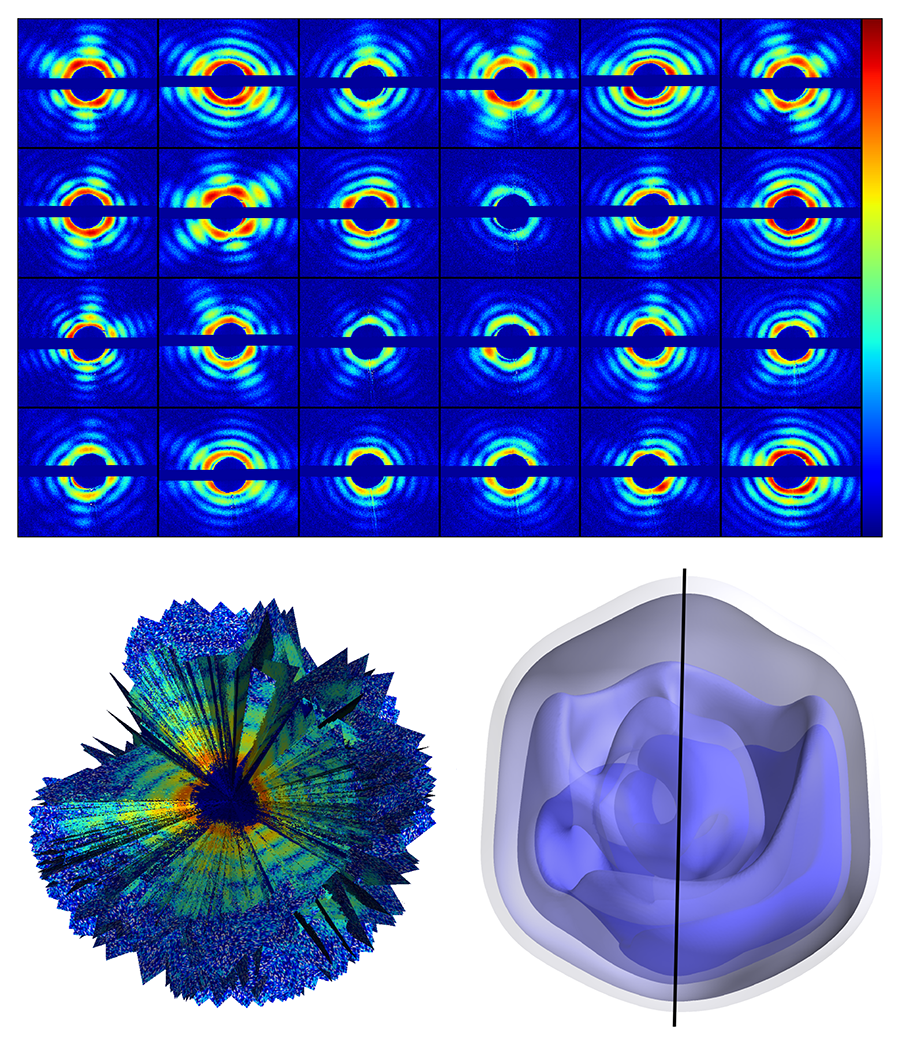
\includegraphics[width=0.5\textwidth]{Figuras/ch1_pulso.png}
  \caption{Patrones de difracción y densidad de electrones obtenida de un \enquote{Mimivirus}\autocite{Ekeberg2015}. La resolución conseguida es de \qty{125}{nm}. El tamaño de la envoltura del virus es aproximadamente de \qty{450}{nm}.}
  \label{fig:ch1_pulso}
\end{figure}

El aspecto clave del ancho de pulso en estas aplicaciones está en conseguir la difracción antes destruir completamente la muestra\autocite{Neutze2000}, motivando la necesidad de pulsos extremadamente cortos o ultracortos ($\le\unit{fs}$) para visualizar imágenes. Por otro lado, el papel de la longitud de onda es conseguir la resolución necesaria para observar menores tamaños, ya que longitudes de onda mayores que el tamaño característico del objeto que quiere estudiarse no permiten exhiben el fenómeno de difracción necesario. En la actualidad ---se explicará más detalladamente en la sección \S\ref{sec:1.3}---, las únicas fuentes de radiación que reúnen estos requisitos son los láseres de rayos X blandos o \emph{\acrfull{sxrl}}.

\section{Plasma}\label{sec:1.2}

\subsection{Propiedades físicas}\label{sec:1.2.1}

\subsection{Ondas electromagnéticas en plasmas}\label{sec:1.2.2}

\subsection{Interacción láser-plasma}\label{sec:1.2.3}

\section{Fuentes de radiación X coherente}\label{sec:1.3}

\subsection{Radiación sincrotrón}\label{sec:1.3.1}

\subsection{Láseres de electrones libres}\label{sec:1.3.2}

\subsection{Armónicos de alto orden}\label{sec:1.3.3}

\subsection{Radiación betatrón}\label{sec:1.3.4}

\section{Láseres de rayos X basados en plasmas}\label{sec:1.4}

\section{Estado del arte}\label{sec:1.5}

\chapter{Objetivos}\label{cap:2}


\chapter{Metodología}\label{cap:3}
\lettrine{P}{ara modelar el proceso de amplificación} de la semilla de armónicos de alto orden introducida a través del canal de plasma, es necesario plantear y resolver numéricamente las denominadas \emph{\acrlong{mbe}} (\acrshort{mbe}). El código Dagon empleado durante las simulaciones implementa estas ecuaciones mediante un programa escrito en Fortran que, a su vez, está acoplado con otros códigos numéricos ---cuya función se explicará más detalladamente en la sección \S\ref{sec:3.2}---, recibiendo información de partida para iniciar el procedimiento de cálculo. De esta forma, los resultados proporcionan los datos necesarios para entender cómo afectan la densidad de iones y electrones libres en el plasma a la intensidad y perfil de fase del haz \acrshort{xuv} obtenido. 

Una vez finalizadas las simulaciones, para poder realizar el análisis de las imágenes y los resultados obtenidos, se emplearon dos nuevos programas ---esta vez escritos en Python y Octave---, que permiten almacenar en un archivo los datos obtenidos en las simulaciones de Dagon y representarlos gráficamente mediante curvas bidimensionales. Además, estos conjuntos de datos pueden introducirse en programas como VisIt para la construcción de imágenes tridimensionales y bidimensionales, por ejemplo, de la propagación del \acrshort{hoh} en la dirección longitudinal del canal.

\section{Ecuaciones de Maxwell-Bloch}\label{sec:3.1}
En este trabajo, el fenómeno físico de la amplificación del armónico inyectado en el plasma de iones de kriptón conduce inevitablemente hasta estas ecuaciones, puesto que determinan cuáles serán las propiedades de la emisión obtenida (\acrshort{ase}). Las \acrshort{mbe} describen la dinámica de la interacción entre los modos de vibración de un campo electromagnético y los átomos de un sistema cuántico con dos estados. 

El formalismo físico-matemático utilizado en mecánica cuántica para obtener las ecuaciones no es trivial\autocite{cohen-tannoudjiQuantumMechanicsVolume2019,cohen-tannoudjiQuantumMechanicsVolume2019a,Sakurai2020,milonniLasers1988}, aunque tiene la ventaja de predecir con suficiente exactitud la evolución temporal del pulso, además de propiedades físicas de los fotones como su momento angular orbital (\acrshort{oam}), mientras que otros métodos más sencillos ---como el programa de trazado de rayos SHADOX--- no ofrecen esta posibilidad, si bien podría utilizarse para resolver el problema de la amplificación en el plasma.

En la interacción láser-plasma estudiada, para obtener una buena aproximación basta considerar el campo eléctrico de la semilla \acrshort{hoh}, aunque cálculos más precisos tendrían que incorporar el acoplamiento del campo magnético. Además, el acoplamiento entre el campo electromagnético y la materia utiliza una aproximación semiclásica simplificada, donde los átomos o iones son sistemas cuánticos de dos estados descritos por la ecuación de Schrödinger, mientras que la luz es un sistema clásico ---una onda electromagnética--- descrito por las ecuaciones de Maxwell.

En primer lugar, el acoplamiento del campo eléctrico con el plasma es la ecuación de ondas 
\begin{equation}\label{eq:3.1}
  \laplacian \symbfcal{E} - \frac{1}{c^{2}}\pdvN{\symbfcal{E}}{t}{2} = \frac{\omega^{2}_{pe}}{c^{2}}\symbfcal{E} + \frac{1}{\epsilon_{0}c^{2}}\pdvN{\symbfcal{P}}{t}{2},
\end{equation}
\noindent
donde el campo eléctrico $\symbfcal{E}$, la polarización $\symbfcal{P}$ y la frecuencia de las oscilaciones del plasma $\omega_{pe}$ son función del espacio y del tiempo.

Para resolver la ecuación, se considera la aproximación paraxial del campo eléctrico según la dirección de propagación del eje $z$. Suponiendo que la radiación está polarizada linealmente en la dirección del eje $x$, esta aproximación permite tener en cuenta únicamente la componente $x$ del campo eléctrico escribiendo por separado la envolvente y las vibraciones del mismo.
\begin{equation}\label{eq:3.2}
  \symcal{E}_{x}(\symbf{r},t) = \RE \left[E_{+}(\symbf{r},t)\eu^{\iu (\omega t - kz)} + E_{-}(\symbf{r},t)\eu^{\iu (\omega t - kz)}\right],
\end{equation}
\noindent
donde $E_{+}$ y $E_{-}$ son la amplitud de las oscilaciones de las ondas viajeras hacia la dirección positiva y negativa del eje $z$, respectivamente. 

Combinando las ecuaciones \eqref{eq:3.1} y \eqref{eq:3.2} y agrupando las componentes que se propagan en las dos direcciones del eje $z$, queda 
\begin{align}
  \laplacian \symcal{E}_{x} 
  &= 
  \left(\pdvN{E_{\pm }}{x}{2} + \pdvN{E_{\pm }}{y}{2} + \pdvN{E_{\pm }}{z}{2} \pm 2k \iu \pdv{E_{\pm }}{z} + k^{2}E_{\pm }\right)\eu^{\iu (\omega t \pm kz)}, \\
  \pdvN{\symcal{E}_{x}}{t}{2}
  &= 
  \left(\pdvN{E_{\pm }}{t}{2} + 2 \omega \iu \pdv{E_{\pm }}{z} + \omega^{2}E_{\pm }\right)\eu^{\iu (\omega t \pm kz)},
\end{align}
\noindent
obteniéndose el lado izquierdo ($\mathrm{LHS}$) de la ecuación de ondas para el campo eléctrico
\begin{equation}\label{eq:3.3}
  \mathrm{LHS} = \left[\laplacian_{\perp}E_{\pm} + \pdvN{E_{\pm }}{z}{2} \pm 2k \iu \pdv{E_{\pm }}{z} - \frac{1}{c^{2}}\left(\pdvN{E_{\pm }}{t}{2} + 2 \omega \iu \pdv{E_{\pm }}{z}\right) 
  -\left(\frac{\omega^{2}}{c^{2}} - k^{2}\right)E_{\pm }\right] \eu^{\iu(\omega t \pm kz)}.
\end{equation}

La ecuación \eqref{eq:3.3} puede reducirse más simplificando la relación de dispersión del campo eléctrico en el plasma $\omega^{2} = \omega^{2}_{pe} + k^{2}c^{2}\approx k^{2}c^{2}$, puesto que para la emisión de radiación \acrshort{xuv} o rayos X blandos ($\lambda<\qty{40}{nm}$) y la densidad electrónica del plasma de kriptón ($n_e<\qty{e21}{cm^{-3}}$) se tiene 
que $\omega>\qty{4,7e16}{rad/s}>\omega_{pe}$ y $\omega_{pe}<\qty{1,8e15}{rad/s}$. Por otro lado, se toma la aproximación de la envolvente lentamente variable (\acrshort{svea}) que asume la variación temporal y espacial de la envolvente del campo eléctrico lenta comparada con la longitud de onda, de manera que
\begin{align}
  \left|\pdvN{E_{\pm }}{z}{2}\right| &\ll \left|k \pdv{E_{\pm }}{z}\right| \ll \left|k^{2}E_{\pm }\right|,\\
  \left|\pdvN{E_{\pm }}{t}{2}\right| &\ll \left|\omega \pdv{E_{\pm }}{t}\right| \ll \left|\omega^{2}E_{\pm }\right|.
\end{align}
\noindent
Introduciendo estas nuevas hipótesis, la ecuación \eqref{eq:3.3} queda
\begin{equation}
  \mathrm{LHS} =
  \left[\laplacian_{\perp}E_{\pm } - \frac{2 \omega \iu }{c^{2}} \left(\pdv{E_{\pm }}{t} \pm c \pdv{E_{\pm }}{z}\right)\right]\eu^{\iu (\omega t \pm kz)}.
\end{equation}

Para la polarización se realiza su descomposición de forma completamente análoga al campo eléctrico.
\begin{align}
    \symcal{P}_{x}(\symbf{r},t) 
    &=
    \RE \left[P_{+}(\symbf{r},t)\eu^{\iu (\omega t -kz)} + P_{-}(\symbf{r},t)\eu^{\iu (\omega t + kz)}\right], \\
    \pdvN{\symcal{P}_{x}}{t}{2}
    &=
    \left(\pdvN{P_{\pm }}{t}{2} + 2 \omega \iu \pdv{P_{\pm }}{z} + \omega^{2}P_{\pm }\right)\eu^{\iu (\omega t \pm kz)}.
\end{align}

Considerando junto a la SVEA que la amplitud de la polarización en un periodo de la onda es mucho mayor que la variación temporal de su envolvente, es decir,
\begin{equation}
  \left|\pdv{P_{\pm }}{t}\right| \ll |\omega P_{\pm }|,
\end{equation}
\noindent
entonces resulta que
\begin{equation}\label{eq:3.4}
  \pdvN{\symcal{P}_{x}}{t}{2} \approx -\omega^{2}P_{\pm }\eu^{\iu (\omega t \pm kz)}.
\end{equation}

La sustitución de las ecuaciones \eqref{eq:3.3} y \eqref{eq:3.4} en la ecuación \eqref{eq:3.1} permite obtener, tras reordenar los términos a izquierda y derecha
\begin{equation}
  \pdv{E_{\pm }}{t} \pm c \pdv{E_{\pm }}{z} = -\iu \frac{c^{2}}{2 \omega}\laplacian_{\perp}E_{\pm } + \frac{\iu \omega}{2} \left[\left(\frac{\omega_{pe}}{\omega}\right)^{2}E_{\pm } - \mu_{0}c^{2}P_{\pm }\right],
\end{equation}
\noindent
obteniendo una ecuación de advección-difusión-reacción con un término fuente $P_{\pm}$ dependiente del espacio y del tiempo. 

Suponiendo que el tiempo característico de expansión hidrodinámica del plasma es mucho mayor que el de evolución de la polarización, la relación constitutiva procedente de las conocidas en mecánica cuántica como \emph{\acrlong{obe}} (\acrshort{obe}) (términos en la diagonal secundaria de la matriz de densidad para la interacción entre el campo eléctrico y un sistema cuántico de dos niveles) es
\begin{equation}
  \pdv{P_{\pm }}{t} = \Gamma - \gamma P_{\pm } - \frac{\iu z^{2}_{12}}{\hslash }E_{\pm }(N_{2}-N_{1}),
\end{equation}
donde $\Gamma$ es un término fuente estocástico que representa la emisión espontánea, $\gamma P_{\pm}$ es un término sumidero que tiene en cuenta la despolarización del plasma debido a colisiones con electrones libres con $\gamma$ el tiempo característico de variación de la polarización, $z_{12}$ es el término de la diagonal secundaria correspondiente a la matriz dipolar eléctrica y $N_{1,2}$ son las poblaciones de los niveles inferior y superior (los de la diagonal principal de la matriz de densidad). Estos elementos se obtienen a partir de las ecuaciones de tasas
\begin{equation}
  \pdv{N_{1,2}}{t} = \sum_{k} C_{k2,k1}N_{k} \pm \frac{1}{2 \hslash }\IM (E_{\pm }^{*}P_{\pm }),
\end{equation}
\noindent
donde el sumatorio recorre todos los niveles energéticos que participan en las transiciones desde un nivel $k$ hasta los dos estados, incluidas las transiciones entre ambos $k=1, 2$ y $C_{ki}$ son las tasas de excitación y desexcitación del sistema debidas tanto a colisiones como a emisión de radiación. Las poblaciones para los niveles $k\neq 1, 2$ y sus tasas se extraen del código OFK para emplear como entrada de Dagon, como se ha comentado antes.

\section{Esquema computacional}\label{sec:3.2}
Los parámetros de entrada sobre el estado del plasma en el momento de la amplificación necesarios para iniciar Dagon proceden de un código llamado OfiKinRad (OFK). Este código simula la interacción a escala atómica de los constituyentes del plasma, aportando datos sobre la temperatura de los electrones, su densidad, la ionización media, la ganancia y las tasas de colisiones entre iones y electrones.

\section{Esquema experimental}\label{sec:3.3}

\section{Parámetros de las simulaciones}\label{sec:3.4}

\chapter{Resultados}\label{cap:4}

\section{Con una sigmoide}

\subsection{Variando el parámetro $r_{i,min}$}

\subsection{Variando el parámetro $k_{i}$}

\subsection{Variando el parámetro $z_{0i}$} 

\subsection{Variando el parámetro \texttt{zshift}}

\section{Con dos sigmoides}

\subsection{Variando el parámetro $r_{ig,max}$}

\subsection{Variando el parámetro $k_{ig}$}

\subsection{Variando el parámetro $z_{0ig}$} 

\section{Con funciones exponenciales}

\subsection{Variando el parámetro $r_{u}$}

\subsection{Variando el parámetro \texorpdfstring{$\sigma_{u}$}{sigma-u}}

\subsection{Introduciendo \acrshort{oam}}

\subsection{Eliminando \acrshort{ase}}


\chapter{Conclusiones}\label{cap:5}



\chapter{Evaluación de impactos}\label{cap:6}

\chapter{Líneas futuras}\label{cap:7}
\lettrine{L}{as posibles perspectivas de futuro} relacionadas con esta línea de trabajo ofrecen distintos caminos, cada uno de los cuales podrían constituir nuevos Trabajos Fin de Grado o Fin de Máster. A partir de los resultados presentados durante el capítulo \S\ref{cap:4}, resumidas en el capítulo \S\ref{cap:5}, existen varias alternativas y combinaciones a explorar para intentar comprender o solucionar algunas de las incógnitas pendientes de resolver completamente: distribución radial de fase y adición del momento angular orbital.

En primer lugar, aunque el acuerdo obtenido entre experimento y simulaciones del perfil radial de intensidad es adecuado, esto sucede debido a que una parte importante de las modificaciones y esfuerzos han sido dedicados a conseguir reproducir la forma de la curva con la mayor precisión posible, mientras que el perfil de fase de los fotones han quedado relegados a un segundo plano, prestando atención simplemente a la formación de la pareja de picos y el valle, simétricamente centrados en la columna de plasma. Sin embargo, la profundidad entre los picos y valle de fase de las simulaciones necesita aproximarse mejor a las observaciones, intentando mantener la distribución de intensidad radial conseguida.

Esta pequeña discrepancia, relativa a la fase de la amplificación ultravioleta extrema (\acrshort{xuv}) obtenida, está relacionada con la introducción de la columna de plasma inicial para el guiado de la semilla de armónicos de alto orden (\acrshort{hoh}) y los pulsos láser en el infrarrojo cercano (\acrshort{nir}). La expansión hidrodinámica del plasma origina un índice de refracción decreciente en dirección radial, esto es, un gradiente de densidad electrónica radial creciente que, en última instancia, es responsable de la distribución de fase de los fotones. Por tanto, futuros trabajos podrían dirigir sus esfuerzos en realizar nuevos cambios del perfil radial de densidad electrónica, utilizando una metodología similar a la empleada para reducir la diferencia entre los máximos y mínimos locales del laboratorio y de las simulaciones.

En segundo lugar, la adición del momento angular orbital (\acrshort{oam}) constituye probablemente el aspecto más interesante a la hora de continuar en futuros trabajos. En general, los resultados obtenidos en combinación con la función exponencial a trozos, introducida para definir la región del canal con \ce{Kr^{8+}}, necesitarán explicarse satisfactoriamente por nuevos estudios. Además, este objetivo podría conseguirse y ampliarse recurriendo, o bien a la introducción del \acrshort{oam} en secciones estudiadas durante el proyecto como, por ejemplo, las sigmoides, o bien mediante otras funciones (recurriendo tal vez a polinomios interpoladores) que puedan reconstruir la frontera de iones \ce{Kr^{8+}} en el plasma.

De este modo, y en línea con el primer punto comentado, también cabría la posibilidad de terminar agrupando estos resultados de intensidad, fase y \acrshort{oam} en un solo sistema de simulación láser-plasma, intentando optimizar otros parámetros como la intensidad máxima del pulso láser infrarrojo \acrshort{nir} a la entrada del columna, la duración de los pulsos participantes, o las características de la semilla \acrshort{hoh} inyectada, tanto intrínsecas como relativas a los demás haces láser, por ejemplo los tiempos de retardo. Así, el objetivo consistiría en mejorar la eficiencia de la conversión de energía ---y la deposición de energía--- tanto del láser \acrshort{nir} de bombeo como durante la amplificación \acrshort{xuv} de la semilla \acrshort{hoh}, que podrían ayudar a capturar de manera más precisa la complejidad de estos sistemas multiescala.

\begin{figure}[htbp]
  \centering
  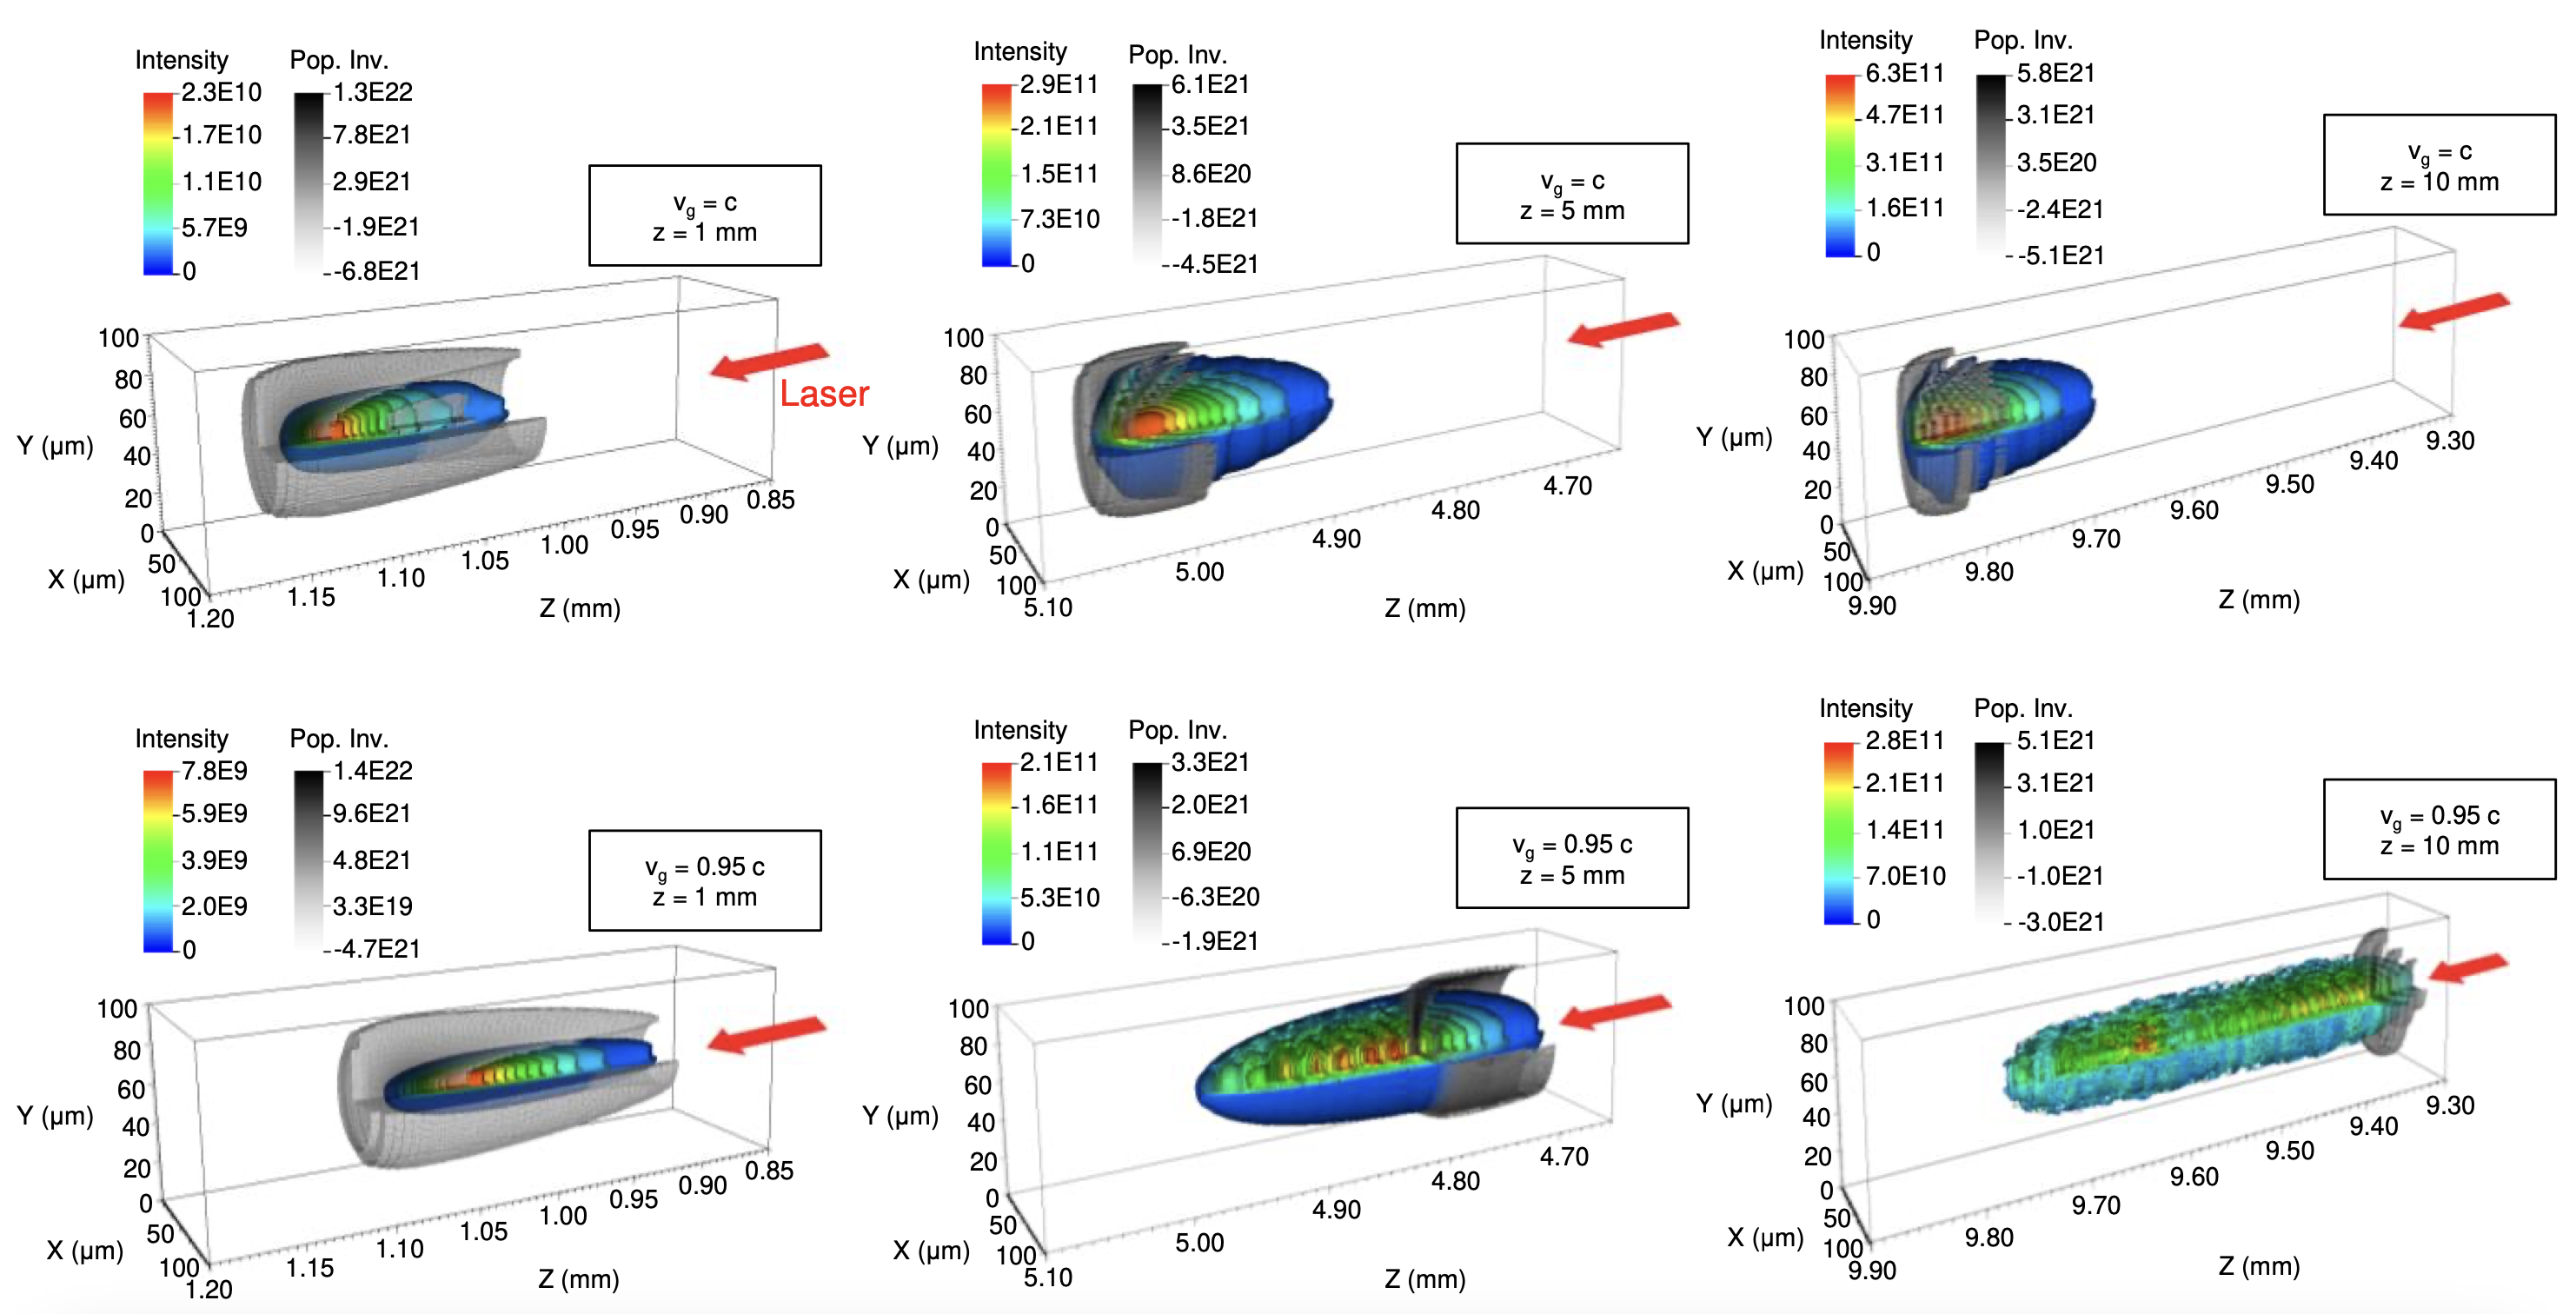
\includegraphics[width=0.8\textwidth]{Figuras/ch7_futuro.png}
  \caption{Simulaciones en tres dimensiones\autocite{Kabacinski2023} con Dagon de la amplificación \acrshort{sxrl} para dos velocidades de grupos distintas, a distintas longitudes de propagación}
  \label{fig:7.1}
\end{figure}

Por último, otra buena región de exploración en posteriores estudios podría incluir la velocidad de propagación de la onda a través del plasma. Aunque no ha sido mencionado anteriormente, existe una desincronización natural entre la semilla \acrshort{hoh} y el pulso \acrshort{nir} de bombeo, producido por las diferentes velocidades de grupo en el interior del plasma. A menor frecuencia, menor velocidad (dispersión negativa), provocando un desacoplamiento entre la semilla \acrshort{hoh} ---que viaja más rápido--- y el haz infrarrojo ---que viaja más lento---, repercutiendo negativamente a la ventana de ganancia. 

Un estudio reciente\autocite{Kabacinski2023} ha demostrado la posibilidad de mejorar la eficiencia de la extracción de energía controlando esta velocidad de grupo, utilizando la secuencia de códigos de este trabajo para simular numéricamente el procedimiento experimental propuesto. El código Dagon incorpora la velocidad de grupo como un parámetro más que puede variarse a voluntad (como muestra la Figura \S\ref{fig:7.1}), permitiendo añadir un grado de libertad adicional a través de la velocidad de la onda, optimizando el fenómeno de la amplificación.

En definitiva, continuar este ámbito de investigación en particular contribuirá a esclarecer su posible interés en investigación, así como en las aplicaciones de formación de imágenes y diagnosis, o en conseguir fuentes de radiación \acrshort{xuv} coherente más pequeñas y eficientes. 


%%% bibliografía
\printbibliography
\chapter{Planificación temporal}\label{cap:9}


\chapter{Presupuesto}\label{cap:10}
\lettrine{D}{urante la realización de este proyecto} han tenido lugar unos costes materiales y personales que pueden cuantificarse y clasificarse en dos grupos diferenciados. Es importante subrayar que, los resultados económicos presentados a continuación consisten en estimaciones aproximadas, basadas en los precios (en promedio) de los recursos empleados, puesto que no ha tenido una asignación presupuestaria o retribución económica asociada. 

Para comenzar, la división de los costes incurridos puede hacerse en directos e indirectos. El primer grupo comprende los gastos relativos a recursos materiales y humanos involucrados en la ejecución del trabajo, mientras que el segundo grupo consiste en gastos de naturaleza variable, principalmente los sistemas de alimentación eléctrica, servicio de conexión a internet y agua caliente sanitaria. Este último grupo está asociado íntegramente a la actividad personal del alumno en su domicilio particular, debido a que la totalidad del proyecto ha tenido lugar a través de un servidor remoto vinculado al Instituto de Fusión Nuclear \enquote{Guillermo Velarde} (IFN-GV). 

Dentro del primer bloque, es posible distinguir distintos tipos de gastos materiales, relacionados simplemente con la amortización de los ordenadores y el coste de las licencias de programas informáticos utilizados. El código Dagon encargado de las simulaciones numéricas (incluyendo todos los programas de Python, Fortran y Octave que participan en Dagon), y el programa VisIt para la obtención de determinadas imágenes, son software libre, por tanto no representan ningún gasto. De este modo, la única licencia a considerar es el paquete institucional de Microsoft $365$ A3 empleada por la Universidad Politécnica de Madrid, con un coste estimado de $100$ € anuales.

Los equipos empleados están formados por el ordenador personal del alumno y el servidor remoto ocupado de ejecutar las códigos numéricos. Teniendo en cuenta la considerable demanda computacional producida, es conveniente considerar un sistema de amortización lineal a $5$ años, extendiéndose a la duración total del trabajo académico (tres cuatrimestres) en ambos sistemas informáticos. El equipo remoto tiene un coste estimado de $4000$ €, mientras que el ordenador particular de $3000$ €. 

La Tabla \ref{tab:10.1} resume los costes directos debidos a los equipos y licencias.

\begin{table}[htpb]
  \centering
  \caption{Costes directos debidos a los recursos materiales.}
  \label{tab:10.1}
  \begin{tabular}{lS}
    \toprule
    Recursos materiales          & {Coste (€)} \\
    \midrule
    Licencia Dagon               & 0           \\
    Licencia VisIt               & 0           \\
    Licencia Microsoft $365$ A3  & 125         \\
    Amortización servidor        & 800         \\
    Amortización portátil        & 600         \\
    TOTAL                        & 1525        \\
    \bottomrule
  \end{tabular}
\end{table}

La Tabla \ref{tab:10.2} muestra los costes directos de las personas que han participado en el proyecto, en este caso, las estimaciones de los salarios brutos del profesor tutor del proyecto (investigador senior, programa de investigación Ramón y Cajal) y el alumno encargado del trabajo. Para simplificar el cálculo del coste horario de las horas de trabajo laborables, es preferible escoger un $28$\% de aportación a la seguridad social sobre los salarios brutos. En la Tabla \ref{tab:10.3}, aparece el coste total de los recursos humanos correspondientes a las horas de dedicación durante los tres cuatrimestres de duración (incluyendo los periodos vacacionales).

\begin{table}[htpb]
  \centering
  \caption{Costes horarios del profesor tutor y el alumno.}
  \label{tab:10.2}
  \begin{tabular}{lSS}
    \toprule
                              & {Alumno} & {Tutor} \\
    \midrule
    Salario Bruto (€/año)     & 8240,5   & 40000   \\
    Seguridad Social (€/año)  & 2307,25  & 11200   \\
    Horas laborales (año)     & 1085     & 1736    \\
    Coste horario (€/hora)    & 9,75     & 29,5    \\
    \bottomrule
  \end{tabular}
\end{table}

\begin{table}[htpb]
  \centering
  \caption{Costes directos del profesor tutor y el alumno.}
  \label{tab:10.3}
  \begin{tabular}{lSSS}
    \toprule
               & {Dedicación (horas)} & {Coste horario (€/hora)} & {TOTAL (€)} \\
    \midrule
    Alumno     & 1356,25              & 9,75                     & 13225       \\
    Tutor      & 125                  & 29,5                     & 3687,5      \\
    TOTAL      & 1481,25              &                          & 16912,5     \\
    \bottomrule
  \end{tabular}
\end{table}

Finalmente, como última hipótesis, los costes indirectos incurridos pueden estimarse suponiendo una contribución del $15$\% sobre el total de los costes directos obtenidos. La Tabla \ref{tab:10.4} recoge los resultados finales, proporcionando un coste final del proyecto de $25655,78$ €.

\begin{table}[htpb]
  \centering
  \caption{Coste total del proyecto.}
  \label{tab:10.4}
  \begin{tabular}{lS}
    \toprule
    Costes totales      & {Coste (€)} \\
    \midrule
    Recursos materiales & 1525        \\
    Recursos humanos    & 16912,5     \\
    Indirectos ($15$\%) & 2765,625    \\
    Sin IVA             & 21203,125     \\
    IVA ($21$\%)        & 4462,65     \\
    TOTAL               & 25655,78    \\
    \bottomrule
  \end{tabular}
\end{table}









%%% índice de figuras y tablas
\listoffigures
\listoftables
\listoflistings

 %%% abreviaturas, acrónimos y símbolos
\printglossary[type=\acronymtype, title=\AUA]

%%% apéndice
\appendix
\chapter{Resultados para una sigmoide}\label{anx:1}


\chapter{Resultados para dos sigmoides}\label{anx:2}




\backmatter

\end{document}
